\subsubsection{Progress}
Over the previous few weeks I have been working on building modules in \texttt{systemverilog} to perform floating point arithmetic so that we can effectively build neural networks on an FPGA. Each layer in the neural network will need to perform this computation to work properly.\newline

The work began with researching how floating point arithmetic is already being done. I had found that the IEEE had already given a standard for double precision floating point binary numbers, that is to say 64 bit floating point numbers in binary. They have also defined single precision (32 bit).\newline

Floating point numbers are structured in a unique way shown below:
\begin{figure}[H]
	\centering
	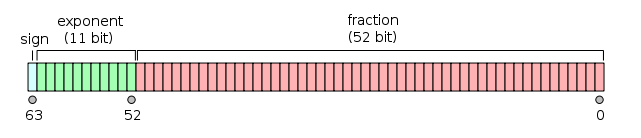
\includegraphics[width=0.85\textwidth]{resources/Double_precision.PNG}
	\caption{Double Precision Floating Point Numbers in Binary according to IEEE 754 Standard}
	\label{fig:double_precision}	
\end{figure}
So the number will be $-1^{sign} \times 2^{exponent - 1023} \times  1.(fraction)$ in the double precision case.\newline
I discovered that modifying the size of the exponent and the mantissa (fraction) would modify the range of accessible numbers and the resolution of the scale respectively. The IEEE 754 standard is far too large for the purpose we need it for and will consume too many Look Up Tables (LUTs) on the FPGA for it to work with the neural network. The alternative I came to was to use half precision floating point numbers (16bit).\newline

After looking up some potential algorithms online I was able to make and compile an Addition, Multiplication, Integer to Floating Point and Floating Point to Integer modules. I have designed the addition module in such a way that it can accept two's compliment 16bit floating point numbers and perform subtraction instead.

\subsubsection{Difficulties Encountered}
The difficulties I encountered were firstly deciding on the size of exponent and the mantissa. Even though the standard is a 5 bit exponent and a 10 bit mantissa, we may have a more optimised structure for the neural networks. For the time being I have simply parameterised the size of the input and the exponent so that it can be changed later and we can discover experimentally which is the best structure for our purpose as we have no known way to find out analytically. \newline

The second difficulty I encountered was writing the test bench. While there are only a handful of cases that are important for each module such as $0+0=0$ and $X \times 0 = 0$, we \textit{do} need to test for a great number of cases (over a million) because if even one calculation yields an erroneous result then the neural networks will not train correctly. It can be quite tedious to hard code each of these cases into the test bench so we had to find a way to have a program correctly calculate the value and correctly convert to 16bit floating point as well as generate a specified number of randomly generated test cases. Once I am confident that these modules work correctly I can make a reciprocal module so that the division operation can be performed. One alternative method I have in mind in the case that the multiplication module does not work in the time frame is to use many addition modules in series for both multiplication and division. 